Let $(a,0)$  and  $(0,a)$ be the intercept points. 
\begin{align}
\vec{m} 
        &=   \myvec{
		a \\
		0 
		} - \myvec{
		   0 \\
		   a
		}  
        		  \equiv \myvec{
                           1 \\
			   -1 
		         } 
			 \\
			 \implies
\vec{n} &=  \myvec{
		     1 \\
		     1
	     } 
\end{align}
and 
the equation of the  line is
\begin{align}
	\myvec { 1 & 1 } \brak{ \vec{ x  - \myvec{ 2 \\
                                   3
			     }
		}}  &= 0  \\
\implies		\myvec{ 1 & 1} \vec{x}  &= 5 
        \label{eq:11/10/2/12/1}
\end{align}
See  \figref{fig:11/10/2/12/Fig1}.
\begin{figure}[H]
	\begin{center}
		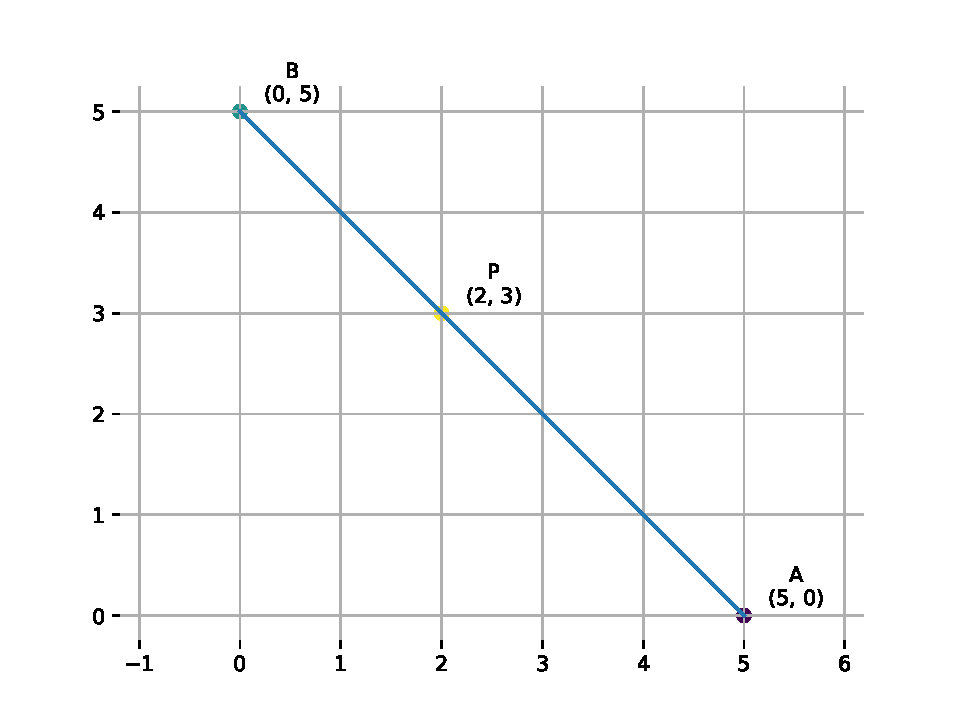
\includegraphics[width=0.75\columnwidth]{chapters/11/10/2/12/figs/fig.pdf}
	\end{center}
\caption{}
\label{fig:11/10/2/12/Fig1}
\end{figure}

